\documentclass{article}
\usepackage[german]{babel}
\usepackage{graphicx,xcolor}

%%%%%%%%%% Start TeXmacs macros
\catcode`\>=\active \def>{
\fontencoding{T1}\selectfont\symbol{62}\fontencoding{\encodingdefault}}
\newcommand{\tminput}[2]{\trivlist{\item[\color{rgb:black,10;red,9;green,4;yellow,2}{#1}]{\color{blue!50!black}\mbox{}#2}}}
\newcommand{\tmoutput}[1]{#1}
\newcommand{\tmsession}[3]{{\tt#3}}
\newcommand{\tmstrong}[1]{\textbf{#1}}
\newcommand{\tmunfoldedio}[3]{\trivlist{\item[\color{rgb:black,10;red,9;green,4;yellow,2}{#1}]\mbox{}{\color{blue!50!black}#2}\item[]\mbox{}#3}}
%%%%%%%%%% End TeXmacs macros

\begin{document}

{\tmstrong{Vorlesung 2 }}19.04.2016

\

\tmsession{shell}{default}{
  \tmoutput{Shell session inside TeXmacs pid = 13978}
  \tminput{Shell] }{g++ -o Vorl2-A3-2 Vorl2-A3-2.cpp \&\& ./Vorl2-A3-2 >
  V2-A3-2-E1.dat\\
  }
  \tminput{Shell] }{g++ -o Vorl2-A3-3 Vorl2-A3-3.cpp \&\& ./Vorl2-A3-3 >
  V2-A3-3-E1.dat\\
  }
  \tminput{Shell] }{g++ -o Vorl2-A3-4 Vorl2-A3-4.cpp \&\& ./Vorl2-A3-4 >
  V2-A3-4-E1.dat\\
  }
  \tminput{Shell] }{\ }
}

\

\tmsession{gnuplot}{default}{
  \tmoutput{This is a TeXmacs interface for GNUplot.}
  \tmunfoldedio{gnuplot] }{ plot 'V2-A3-2-E1.dat' using 1:2 pt 7 ps
  0.5}{\raisebox{0.0\height}{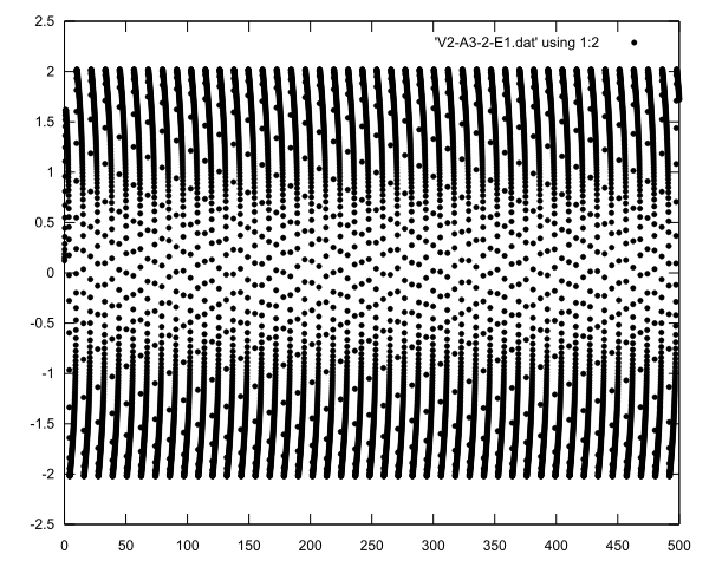
\includegraphics[width=11.89935064935065cm,height=9.519480519480519cm]{Vorlesung-2--1.pdf}}}
  \tmunfoldedio{gnuplot] }{plot 'V2-A3-3-E1.dat' using 1:2 pt 7 ps
  0.5}{\raisebox{0.0\height}{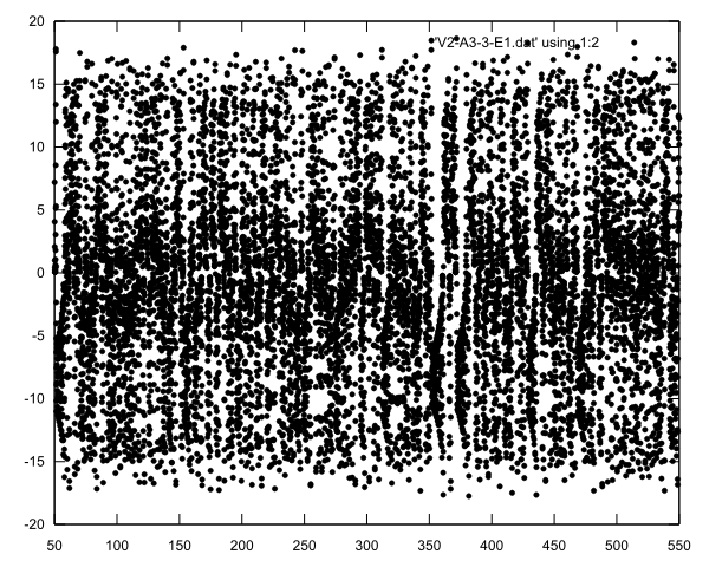
\includegraphics[width=11.89935064935065cm,height=9.519480519480519cm]{Vorlesung-2--2.pdf}}}
  \tmunfoldedio{gnuplot] }{plot 'V2-A3-4-E1.dat' using 1:2 pt 7 ps
  0.5}{\raisebox{0.0\height}{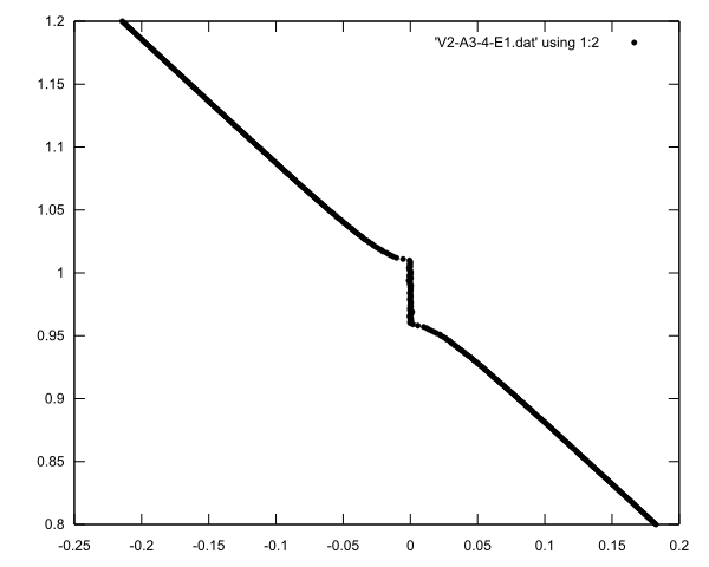
\includegraphics[width=11.89935064935065cm,height=9.519480519480519cm]{Vorlesung-2--3.pdf}}}
  \tminput{gnuplot] }{\ }
}

\end{document}
